%%--------------------Chapter 3------------------------
\chapter{Hybrid Systems Preliminaries}\label{chap:hybrid}

\section{Theoretical Foundations of Hybrid Systems}

\subsection{Formalism of a Hybrid System}

Dynamical systems are mathematical models that capture the evolution of a set of variables over time (which can be continuous or discrete) with respect to given initial conditions. The set of variables, excluding time, collectively defines the state space of the system. Dynamical systems are traditionally classified into two categories, based on the nature of the state space -- continuous dynamical systems and discrete dynamical systems. However, there is a category that subsumes both types of dynamical systems while also extending them -- hybrid dynamical systems, or more commonly referred to as hybrid systems.
Hybrid systems have a heterogeneous state space that contains both discrete and continuous variables, with complex evolution equations that make use of coupled discrete and continuous dynamics, non-determinism, and other constructs like differential inclusions or differential-algebraic equations. This generality makes hybrid systems capable of modeling a wide range of complex behaviors, but can often result in ambiguous semantics and challenging analysis. 
% Given the ubiquity of discrete jumps in hybrid systems, their trajectories are often discontinuous.

\subsection{Hybrid Systems as Hybrid Automata}

Hybrid automata are the conventional formalism for representing hybrid systems. Hybrid automata use a  state machine representation, where discrete states (also referred to as \textit{locations}) represent the set of discrete-valued variables. Transitions between locations represent a change in the value of the underlying discrete-valued variable. Each location is also endowed with a set of continuous variables and a vector field that defines the time evolution of the continuous set. Time is conventionally continuous-valued and the vector field is often an autonomous system (not explicitly dependent on time).

More formally, a hybrid automaton is a tuple $\mathbb{H} = \\(Q, I, \Sigma, Y, F, T, G, R)$ consisting of the components:

State space: $Q = L \times X$,where $L$ is a finite set of locations and $X$ is the set of continuous variables. Each state can be described by $(l,x) \in Q$, where $l \in L$ and $x \in \mathbb{R}^n$.

Initial condition: $I = (l_0,x_0) \in Q$, the state of the system at time $t = 0$

Events: $\Sigma$ is the finite alphabet or event set of $\mathbb{H}$. Let $\Sigma$ always contain the \textit{empty label} or $\zeta$.

Outputs: $Y$ is the output space of $\mathbb{H}$, which may consist of both continuous and discrete elements.

Continuous Dynamics: $F$ is a function on $L$ assigning a vector field or differential inclusion to each to each location in the automaton.

%Invariant conditions: $I \subset 2^X$ is a set of invariant conditions on the continuous states, one for each location $l$ in $L$.

Transitions: $T \subset L \times \Sigma \times L$ is a set of directed edges. $t = (l,\sigma, l') \in T$ is a directed edge between a source location $l \in L$ and a target location $l' \in L$ with event label $\sigma \in \Sigma$. For any $t$ with event label not explicitly given, let the event be labelled with the empty label $\zeta$. In addition, $T = T_{\Theta} \cup T_{U}$, where $T_{\Theta}$ is the set of \textit{forced} transitions while $T_{U}$ is the set of \textit{unforced} transitions. Forced transitions take place instantaneously when the associated guard condition is crossed, while unforced transitions fire non-deterministically after the guard condition is crossed. That is to say, unforced transitions can take place at any time when the guard condition holds true, but are not required to. Unforced transitions may not fire at all.

% a transition may have one of more guards
% union of inequalities becomes guard space
% 
Guard conditions: $G \subset 2^X \times T$ is the set of guard conditions for each transition $t \in T$. The shorthand $G(t) = g_t \in 2^X$ is used to associate a guard condition with its transition. If no $g_t$ is explicitly given for some transition $t \in T$, then its default value is taken to be $X = R^n$. % guard is always valid

Reset conditions: $R$ is the set of reset conditions for each transition $t \in T$. The shorthand $R(t) = r_t$ is used, where $r_t : X \Rightarrow 2^X$ is a set-valued map. If no $r_t$ is explicitly specified for some transition $t \in T$, then the default value is taken to be the identity function for all $x \in X$.

\subsection{Simulation, Bisimulation, and Languages over Automata}

Define the set of \textit{trajectories} of some hybrid automata $\mathbb{H}$ as $\Omega(\mathbb{H})$. While trajectories are a well-formalized concept in the area of continuous dynamical systems, there are several conflicting definitions in the hybrid systems literature, so to be explicit, a trajectory of some hybrid automaton $\mathbb{H}$ is a \textit{continuous trace} of the output space $\mathbb{H}_Y$. A continuous trace $f$ of some variable $x$ means that for each $t \in \mathbb{R}^+$, $f(x,t) = x_t$; that is, $x$ has value $x_t$ at time $t$. Note that there is no condition that the function $f$ itself be continuous; hybrid automata often possess discontinuous jumps induced by resets, so $\text{lim}_{t \rightarrow t_1} \; f(x, t) \neq f(x, t_1)$ upon some transition (and reset $x = c_1$) at time $t_1$.  A continuous trace can also be defined for an arbitrary set of variables $X = \{ x_1, x_2, ... \}$ such that $f(X,t) = \{ f(x_1, t), f(x_2, t), ... \}$. Hence, a continuous trace of the output space $\mathbb{H}_Y$ is given by some function $f(\mathbb{H}_Y, t) = \{ f(y_1, t), f(y_2, t), ... f(y_{|\mathbb{H}_Y|}, t) \}$. 

Two trajectories $f_1(\mathbb{H}_Y, t)$ and $f_2(\mathbb{H}_Y, t)$ are considered equivalent if and only if, for each $f_1(\mathbb{H}_Y, t_1)$ and $f_1(\mathbb{H}_Y, t_2)$ where $t_1 < t_2$, there exists a $t^{'}_1 , t^{'}_2 \in \mathbb{R}^+$ where $f_1(\mathbb{H}_Y, t_1) = f_2(\mathbb{H}_Y, t^{'}_1)$ and $f_1(\mathbb{H}_Y, t_2) = f_2(\mathbb{H}_Y, t^{'}_2)$ and $t^{'}_1 < t^{'}_2$. Note that $t_1, t_2$ do not have to equal $t^{'}_1 , t^{'}_2$ for the previous relation to hold; two trajectories are equivalent if both trajectories contain the same terms and the order in which the terms appear is the same. Hence, trajectories are \textit{time-scale invariant}; $f(\mathbb{H}_Y, t)$ is equivalent to $f(\mathbb{H}_Y, ct)$ for all positive \textit{c} under the previous relation. 

Denote that two trajectories $f_1, f_2$ are equivalent by $f_1 \equiv f_2$. The relation $\equiv$ defines an equivalence class over the set of trajectories $\{ f(X,t) \}$, where $X = \{x_1, x_2, ...\}$. Trajectories themselves can belong to the same equivalence class even if they originate from different hybrid automata, so long as $\mathbb{H}_{1_Y}$ and $\mathbb{H}_{2_Y}$ contain the same elements.

A hybrid automaton $\mathbb{H}_1$ is said to \textit{simulate} another hybrid automaton $\mathbb{H}_2$ if $\mathbb{H}_{1_Y} = \mathbb{H}_{2_Y}$ and for each trajectory $f_2(\mathbb{H}_{2_Y}, t) \in \Omega(\mathbb{H}_2)$, there exists $f_1(\mathbb{H}_{1_Y}, t) \in \Omega(\mathbb{H}_1)$ such that $f_1(\mathbb{H}_{1_Y}, t) \equiv f_2(\mathbb{H}_{2_Y}, t)$. Note that this does not imply that $\mathbb{H}_{1_X} = \mathbb{H}_{2_X}$ or even that $\Omega(\mathbb{H}_2) \subset \Omega(\mathbb{H}_1)$. It simply states that every trajectory taken by $\mathbb{H}_2$ has an equivalent trajectory in $\Omega(\mathbb{H}_1)$ \textit{under the output space} $\mathbb{H}_{1_Y} = \mathbb{H}_{2_Y}$. If the output space $\mathbb{H}_{1_Y} \subset \mathbb{H}_{1_X} + \mathbb{H}_{1_L}$ is ``widened" to include more elements of $\mathbb{H}_{1_X} + \mathbb{H}_{1_L}$, $\mathbb{H}_1$ may not necessarily simulate $\mathbb{H}_2$ under this new shared output space. Denote that $\mathbb{H}_1$ simulates $\mathbb{H}_2$ by $\mathbb{H}_2 \subset \mathbb{H}_1$. If $\mathbb{H}_2 \subset \mathbb{H}_1$ and $\mathbb{H}_1 \subset \mathbb{H}_2$, they are said to \textit{bisimulate}. Denote bisimulation by $\mathbb{H}_1 \equiv \mathbb{H}_2$. Bisimulation defines an equivalence relation (and hence equivalence classes) over the set of hybrid automata with the same output space. Denote the set of hybrid automata with some output space $Y$ as $\{ \mathbb{H}(Y) \}$. Hence, all hybrid automata belong to one (and only one) set of the form $\{ \mathbb{H}(Y) \}$ and equivalence classes are defined over the set of all hybrid automata. From the above, an ontology of hybrid automata can be constructed. The set of all hybrid automata can be broken up into sets of hybrid automata $\{ \mathbb{H}(Y_1) \}, \; \{ \mathbb{H}(Y_2) \}, ...$ with output spaces $Y_1, Y_2, ...$ and each set $\{ \mathbb{H}(Y_i) \}$ is divided into equivalence classes by the bisimulation relation $\equiv$.

\section{Formal Verification of Hybrid Automata}

The formal verification of a hybrid automaton $\mathbb{H}$ involves checking the satisfaction of some predicate, $p$, over the set of continuous traces $\{ f(\mathbb{H}_X + \mathbb{H}_L, t) \}$. The set of traces $\{ f(\mathbb{H}_X + \mathbb{H}_L, t) \}$ is used instead of the set of trajectories $\Omega(\mathbb{H})$ as any predicate over the trajectories restricts $p$ to the variables defined in the output space $\mathbb{H}_Y$. Invoking the operators of modal logic, $p$ is a safety property if the satisfaction condition for $p$ is $ \Diamond p$, while $p$ is a liveness property if the satisfaction condition for $p$ is $\Box p$.

The term \textit{formal verification}, as it will be used henceforth, refers to the computation of the \textit{reachable set} of some $\mathbb{H}$ such that that the predicate $\Box p \; | \; \Diamond  p$ is evaluated as $true$ or $false$. The reachable set of $\mathbb{H}$ is equivalent to $lim_{t \rightarrow \infty} \{ f(\mathbb{H}_X + \mathbb{H}_L, t) \}$. The \textit{reachability problem} for $\mathbb{H}$ is defined as $\exists f \in lim_{t \rightarrow \infty} \{ f(\mathbb{H}_X + \mathbb{H}_L, t) \} \; | \; \Diamond p \; [f]$.

The \textit{finite-time reachability problem} is of particular interest given the computational difficulty of precisely computing the reachable set for the general class of hybrid automata. The finite-time reachable set is given as $\Big\{ \{ f(\mathbb{H}_X + \mathbb{H}_L, t) \}, \; \forall t \in [0, t_{\text{end}}] \Big\}$ and the associated reachability problem is defined as $\exists f \in \Big\{ \{ f(\mathbb{H}_X + \mathbb{H}_L, t) \}, \; \forall t \in [0, t_{\text{end}}] \Big\} \; | \; \Diamond p \; [f]$.


\subsection{Hybrid Automata and Decidability}

The reachability problem is exactly decidable for a small subclass of hybrid automata. A precise boundary between decidable automata and undecidable was theoretically established by Henzinger et al. Furthermore, the results of Collins and Lygeros showed that the finite-time reachable set cannot always be approximated to an arbitrary level of precision. Hence, numerically-sound (under/over)-approximation techniques for reachable set computation must be developed to provide answers to the finite-time reachability problem for the general class of hybrid automata.

\subsection{Taylor Models and Flowpipe Construction}

One of the more promising techniques for finite-time reachable set computation involves approximating the automaton dynamics with \textit{Taylor models}. Taylor models are a robust and generalizable framework for approximating a function by its Taylor series coupled with a symbolic remainder interval. They are useful in particular for verifying hybrid automata as there are few numerically-sound techniques for doing so when the automata in question contain nonlinear dynamics. Approximating a function with a Taylor model of degree \textit{k} requires the function to be continuous and \textit{k}-times differentiable. Conventional operations on functions, like addition, subtraction, composition, and integration are preserved under Taylor model approximation. The working definition of Taylor models and the associated operations in the elucidation to follow is provided by Berz and Makino, as expounded on by Chen et al. The theory of flowpipe construction is provided by the works of Chen et al. This section is intended to provide a high-level overview of the theory of Taylor models using the canonical definition that is familiar to researchers working in the area. Divergent formulations of Taylor models and deviations from the theory will be noted when they arise in the sections to come.  %Hence, nonlinear dynamics like ${ dx/dt = e^t + cos(x) \; log(t) }$ can be represented as $dx/dt = TM(e^t + cos(x) \; log(t), k)$ as $\int^s_{t=0} e^t + cos(x) \; log(t) \; dt \in \int^s_{t=0} TM(e^t + cos(x) \; log(t), k) \; dt$. 

The Taylor approximation of a function $f, \; D \rightarrow \mathbb{R}, \; D \subset \mathbb{R}^n$ with degree $k$ is given as the polynomial $p$ where $p(x_{*}) = f(x_{*})$ for the central point $x_{*} \in D$ and for $1 \leq j \leq k, \; 1 \leq i \leq n, \; \partial^j f(x_{*}) / \partial x^j_i = \partial^j p(x_{*}) / \partial x^j_i$. A necessary and sufficient condition for the existence of $p$ is that all partial derivatives of $f$ with degree \textit{k} exist and are themselves continuous, denoted by $f \in \mathbb{C}^k$. For any $f, g \in \mathbb{C}^k, \; f \equiv_k g$ iff there exists a polynomial $p$ that is the Taylor approximation of both $f$ and $g$. Hence, the Taylor approximation partitions $\mathbb{C}^k$ into a collection of equivalence classes.

Let $\mathbb{I}$ denote the set of all intervals $[l, u], \; l \leq u, \; l, u \in \mathbb{R}$. Intervals in $\mathbb{R}^n$ are given as hyper-rectangles and are elements of the set $\mathbb{I}^n = \mathbb{I} \times \mathbb{I} \times ... \times \mathbb{I} = \prod^n_{i=1} \mathbb{I}$.

A Taylor model (TM) of degree \textit{k} over the domain $D \subset \mathbb{R}^n$ is a 2-tuple $(p, I)$ where $p$ is a polynomial of degree \textit{k} over $n$ variables and $I$ is a remainder interval $I \in \mathbb{I}$. Denote a Taylor model with degree \textit{k} of the function $f, \; D \rightarrow \mathbb{R}$ by $TM(f, k) = (p, I)$ where $p$ is the Taylor approximation of $f$ with degree $k$. Some $(p, I)$ is a \textit{bounded over-approximation} $f \in \mathbb{C}^k$ wherein $\forall x \in D, f(x) \in p(x) + I = \{ p(x) + y \; | \; y \in I \}$.

As polynomials can be generalized to vectors of polynomials to approximate vector-valued real functions of the form $f, \; D \rightarrow \mathbb{R}^m$, Taylor models can be constructed for functions $f$ insofar as they remain \textit{k}-times differentiable for all partial derivatives. A \textit{k}-degree Taylor model of $f$ is given as $TM(f,k) = (p, I)$ where $I \in \mathbb{I}^m$.

To find the trajectory $\overline{X}(t)$ for some $d\overline{X} / dt = F(\overline{X}, t)$ with respect to the initial condition $x_0$, the \textit{flow map} $\phi$ should be computed wherein $\overline{X}(t) = \phi(x_0)(t)$. The flow map defines the set of trajectories reachable from $ x_0 \in X_0$ at time $t$ and ${ \{ \phi(x_0, t'), \; \forall x_0 \in X_0, \; \forall t' \in [0,t] \} }$ is the reachable set at time $t$. However, many $d\overline{X} / dt$ do not have a closed-form solution $\phi$ that can be directly solved for. Hence, the calculation (and representation) of $\phi$ is an ideal domain for the application of Taylor models. For some dynamical system $f = d\overline{X} / dt$, denote the degree \textit{k} Taylor model of its flow map $\phi_f$ by $FM(f, k) = TM(\phi_f, k) = (p, I)$, where $p$ is the degree \textit{k} polynomial and $I$ is the symbolic interval of the Taylor model, both satisfying the necessary differentiability and over-approximation conditions with respect to $\phi_f$. 

There are two primary approaches to compute the polynomial $p$ in $FM(f,k)$ for $f \in \mathbb{C}^k$. The first uses finite iterations (in fact, at most $k$ are needed) of the \textit{Picard operator} with the polynomial $p$ as its fixed point. 

Given some differential equation $d\overline{X} / dt = F(\overline{X}, t)$ and a function $g(x_0, t)$ where $x_0 \in \overline{X}$, the Picard operator is defined as: 
\[ \mathbb{P}_F(g)(x_0, t) = x_0 + \int^t_{s=0} F(g(x_0, s), s) ds \]

If $F$ is Lipschitz continuous, $\mathbb{P}_F$ has a unique fixed point $g_*$ that is the solution $\overline{X}(t)$ to $d\overline{X} / dt = F(\overline{X}, t)$ with initial condition $x_0$ and successive iterations of the Picard operator are guaranteed to converge to $g_*$. More rigorously: 
\[ \mathbb{P}_F(\mathbb{P}_F...\mathbb{P}_F(\mathbb{P}_F(g)))(x_0, t) = \text{lim}_{n \rightarrow \infty} \; \mathbb{P}_F^n(g)(x_0, t) = g_* \]

To find the polynomial $p$ for $FM(f,k)$, truncated iterations of the Picard operator $\mathbb{P}_f$ are applied such that the terms of degree greater than $k$ are dropped after each iteration. This process is guaranteed to converge, given the convergence of the non-truncated Picard iterations when $F = f$.

As an example, take the differential equation $dx/dt = x^3 + 1$ with initial condition $x_0 = 1$. This is known to have closed-form solution $t + \frac{1}{18} (\sqrt{3} \pi + 6 \; \text{log}(2)) = \frac{tan^{-1}( \frac{2 x(t) - 1} {\sqrt{3}} )} {\sqrt{3}} + \frac{1}{3} \; \text{log}(1 + x(t)) - \frac{1}{6} \; \text{log}(x(t)^2 - x(t) + 1)$. This is challenging to compute even with prior knowledge of its form and unwieldly to work with because of the difficulty of isolating $x(t)$. Hence, this is an excellent candidate to showcase the power of Taylor model integration. The polynomial $p$ for the Taylor model $FM(x^3 + 1, 3)$ will be calculated. To calculate the first Picard iterate, set $g_0 = 1$ and $F = x^3 + 1$. Then, $\mathbb{P}_F(g_0)(1, t) = 1 + \int^t_{t=0} (1^3 + 1) \; dt = 2t + 1$. $\mathbb{P}_F^2(g_0)(1, t) = \mathbb{P}_F(g_1)(1, t) = 1 + \int^t_{t=0} ((2t + 1)^3 + 1) \; dt = 1 + 2 t + 3 t^2 + 4 t^3 + 2 t^4$. This process is iterated until the truncated iterates converge, as demonstrated in the table below:

\begin{figure}[!h]
    \centering
  \begin{tabular}{|c|c|c|}
    \cline{2-3}
    \multicolumn{1}{c|}{} & Picard iterate & Expanded terms \\ \hline
        $g_1 = \mathbb{P}_F(g_0)(1, t)$ & $1 + \int^t_{t=0} (g_0^3 + 1) \; dt$ & 2t + 1 \\ \hline 
        $g_2 = \mathbb{P}^2_F(g_0)(1, t)$ & $1 + \int^t_{t=0} (g_1^3 + 1) \; dt$ & $2 t^4 + \mathbf{4 t^3 + 3 t^2 + 2 t + 1}$  \\ \hline 
        $g_3 = \mathbb{P}^3_F(g_0)(1, t)$ & $1 + \int^t_{t=0} (g_2^3 + 1) \; dt$ & $\scriptstyle\frac{8 t^{13}}{13} + 4 t^{12} + 12 t^{11} + \frac{116 t^{10}}{5} + 34 t^9 + \frac{81 t^8}{2} + \frac{279 t^7}{7} + 33 t^6 + \frac{117 t^5}{5} + 14 t^4 + \mathbf{7 t^3 + 3 t^2 + 2 t + 1}$  \\ \hline 
        $g_4 = \mathbb{P}^4_F(g_0)(1, t)$ & $1 + \int^t_{t=0} (g_3^3 + 1) \; dt$ & $\scriptstyle\frac{64 t^{40}}{10985}+\frac{256 t^{39}}{2197}+\frac{192 t^{38}}{169} + \; ... \; +\frac{4887
t^8}{14}+\frac{6129 t^7}{35}+\frac{837 t^6}{10}+\frac{189 t^5}{5}+\frac{65 t^4}{4}+ \mathbf{7 t^3+3 t^2+2 t+1}$ \\ \hline 
  \end{tabular}
    \end{figure}Convergence is achieved upon the third iteration and $p = 7t^3 + 3t^2 + 2t + 1$ for $p \in FM(x^3 + 1, 3)$. For the special case that $f$ contains nonpolynomial terms, e.g. $FM(\frac{cos(x)}{e^x}, 5)$, an approximate polynomial term should be used to replace them before the Picard iterates are computed. In the previous scenario, $cos(x)$ and $e^x$ would be replaced with their own Taylor polynomials, which then allow $\mathbb{P}_f(g_0)(x_0, t)$ to be computed as an integral of polynomial terms.\newline
    
    

The second approach to compute the polynomial $p$ for a flowmap uses a truncated \textit{Lie series} built from the \textit{Lie derivatives} $\mathcal{L}, \mathcal{L}^2, ..., \mathcal{L}^k$. The Lie derivative of some function $g(\overline{X}, t)$ is $\mathcal{L}_F(g)(\overline{X}, t) = \partial g(\overline{X}(t), t) / \partial t$ where $\overline{X}(t)$ is some trajectory and $d\overline{X} /dt = F(\overline{X}, t)$. The Lie derivative is given by:
\[ \mathcal{L}_F(g) = (\nabla_{\overline{X}} \; g) \cdot F(\overline{X}, t) + \partial_t \; g = (\nabla_{\overline{X}} \; g) \cdot d\overline{X} /dt + \partial_t \; g \] 

For some dynamical system $d\overline{X} / dt = F(\overline{X}, t)$, a locally unique solution $\overline{X}(t)$ from the initial condition $x_0$ is given by $\overline{X}(t) = \phi(t, x_0)$, where $\phi(t, s) = \text{lim}_{k \rightarrow \infty} \Sigma^k_{i=0} \frac{t^i}{i!} \mathcal{L}^i_f (x)(s,0)$.


Assembling the previous, the polynomial $p$ for some $FM(f,k)$ is the truncated Lie series around $(x_0, 0)$: 
\[ p = \Sigma^k_{i=0} \frac{t^i}{i!} \mathcal{L}^i_f (x) (x_0,0) = x_0 + t\mathcal{L}_f (x) (x_0,0) + \frac{t^2}{2} \mathcal{L}^2_f (x) (x_0,0) + ... + \frac{t^k}{k!} \mathcal{L}^k_f (x) (x_0,0) \] As before, $p \in FM(x^3 + 1, 3)$ will be computed as an example: \newline

  \begin{tabular}{|c|c|}
    \cline{2-2}
    \multicolumn{1}{c|}{} & Lie derivative \\ \hline
        $\mathcal{L}_f (x)$ & $1+x^3$ \\ \hline 
        $\mathcal{L}^2_f (x) = \mathcal{L}_f (1+x^3)$ & $3 x^2 + 3 x^5$  \\ \hline
        $\mathcal{L}^3_f (x) = \mathcal{L}_f (3 x^2 + 3 x^5)$ & $6 x + 21 x^4 + 15 x^7$  \\ \hline 
        $\mathcal{L}^4_f (x) = \mathcal{L}_f (6 x + 21 x^4 + 15 x^7)$ & $6 + 84 x^3 + 105 x^6 + 105 x^9$  \\ \hline 
  \end{tabular}  \newline\newline The first four Lie derivatives are assembled into a Lie series as follows: \newline$ \Sigma^4_{i=0} \frac{t^i}{i!} \mathcal{L}^i_f (x) = x + (1+x^3)t + (3 x^2 + 3 x^5)\frac{t^2}{2} + (6 x + 21 x^4 + 15 x^7)\frac{t^3}{3!} + (6 + 84 x^3 + 105 x^6 + 105 x^9)\frac{t^4}{4!} = t + \frac{t^4}{4} + x + t^3 x + \frac{3 t^2 x^2}{2} + t x^3 + \frac{7 t^4 x^3}{2} + \frac{7 t^3 x^4}{2} + \frac{3 t^2 x^5}{2} + \frac{35 t^4 x^6}{8} + \frac{5 t^3 x^7}{2} + \frac{35 t^4 x^9}{8}$. \newline\newline This series is then evaluated at $x = x_0 = 1$, rendering $\mathbf{1 + 2 t + 3 t^2 + 7 t^3} + (25 t^4)/2$. None of the $\mathcal{L}(x)... \mathcal{L}^4(x)$ need be evaluated at zero as they each contain no $t$ terms due to the autonomous differential equation. Note that the terms with degree 3 or less are the same as those received from the Picard iterations. Hence, $p = 1 + 2 t + 3 t^2 + 7 t^3$.

In the case that $x$ in $\mathcal{L}_f (x)$ is vector-valued, e.g. $x = \overline{X}$, $m$ polynomials $p_1, ..., p_m$ must be calculated wherein each Lie series is respectively built with the Lie derivatives $\mathcal{L}_{f} (\overline{X}_j), \; 1 \leq j \leq m$, giving the solution $\overline{X}(t) = [p_1(t), ..., p_m(t)]$. This is because the gradient operator $\nabla_{\overline{X}}$ is not defined for a $g = x$ that is already vector-valued.

The second part of computing the Taylor model for a flowmap $FM(f, k)$ involves computing the symbolic interval $I$. To review, the interval $I$ should be established such that $p(x_0, t) - \phi_f(x_0, t) \in I, \forall t \in [0, \Delta]$. The interval $I$ can be computed by guessing a sample $I_0$ and applying the Picard operator on $p' = p + I_0$ to obtain $p''$. If $p'' - p \subset I_0$, $I_0$ is a valid interval and $FM(f, k) = (p, I)$ is a valid overapproximation of $\phi_f(x_0, t)$. This relationship holds because $p'' - p \subset I_0$ means the Picard operator is \textit{contractive} on $I_0$. The interval can be tightened by repeatedly applying the Picard operator to achieve a series of $p'', p''', ..., p^n$ until the relationship $p_n - p \subset I_n$ no longer holds. In the event that $p'' - p \not\subset I_0$, a bigger initial $I$ must be chosen such that $I_0 \subset I_1$. 

Using the theory of flowmaps, an overapproximation of the reachable set for the continuous system $d\overline{X} / dt = F(\overline{X}, t)$ can be computed as follows, with respect to the initial set $X_0$ and total time $t$:

\begin{enumerate}
    \item Pick some interval $[0, \delta_1] \subset [0, t]$
    \item Calculate the \textit{k}-degree flowmap $FM(d\overline{X} / dt, k)$ with respect to the initial condition $x_0 \in X_0$
    \item Compute the reachable set $X_1 = \{ p(x_0)(t) + I, \; \forall t \in [0,\delta], \; \forall x_0 \in X_0 \}$
    \item Pick another interval $[0, \delta_2]$ such that $[0, \delta_1 + \delta_2] \subset [0,t]$
    \item Repeat steps 2-3 over this interval to achieve the set $X_2$
    \item Pick an interval $[0, \delta_i]$ where $[0, \delta_1 + ... + \delta_{i-1} + \delta_{i}] \subset [0,t]$ and iterate steps $2-3$ \textit{n} times until $\delta_1 + ... + \delta_{n-1} + \delta_{n} = t$ and set $X_n$ is achieved
    \item Set $X_n$ is the reachable set from $X_0$ over $[0,t]$
\end{enumerate}


Smaller intervals $\delta_1, ..., \delta_n$ and higher degree Taylor models will result in a more accurate approximation of the reachable set. The size of the interval may be fixed $\delta_1, ..., \delta_n = \delta$ or may be determined on-the-fly within each iteration, with considerations made to the specific dynamic properties of the interval. Taylor model terms of high degree may be dropped between iterations as is often necessary to keep the overall degree of the approximation within a manageable upper bound.

It is important to note that Taylor models map the domain to a set of bounded regions in the codomain. Hence, Taylor models are able to provide a bounded overapproximation of the range of a wide variety of functions, and as shown before, can be used to provide guaranteed enclosures to the solution of most ordinary differential equations. In practice, they have been shown to produce sound results for the trajectories of complex dynamical systems and do not lose numerically stability across long time-scales. Hence, Taylor models serve as a strong foundation for computing reachable sets for the general class of hybrid automata.

However, the integration of Taylor models alone is not enough to simulate the trajectories of hybrid automata. Specifically, the intersection of the integrated Taylor models (henceforth referred to as the \textit{flowpipe}) and the guard conditions must be calculated in order to determine transition times.

%rewrite, this is verbatim.

Taylor models and guard conditions

\subsection{Other Common Approaches}

NuXMV

Hybrid automata with affine approximations

Differential dynamic logic

\subsection{The Ariadne C++ Library}

\subsection{Theoretical Foundations of Ariadne}

Ariadne is based on the theory of \textit{computable analysis}, which seeks to provide a rigorous foundation for functions of a real-variable within a discrete, circuit-level representation. As the reals $\mathbb{R}$, their positive restriction $\mathbb{R}^+$ and the real vector spaces $\mathbb{R}^n, n \in \mathbb{N}$ have continuum cardinality, there is no direct way to map their structure into a discrete interval, such as that given by the 32 or 64-bit floating point numbers.  The naive approach -- taking a finitization of the uncountable set such that it maps onto the discrete structure -- is not mathematically rigorous under the standard operations over the reals. A symbolic representation, then, may seem desirable, that avoids the truncation errors induced by the previous approach, but symbolic operations quickly become memory-and-CPU intensive and unwieldly for serious computation. The theory of \textit{computable analysis} seeks to remedy both of these issues by providing rigorous representations of real numbers and their functions without sacrificing computational efficiency.

Computable analysis represents the set $\mathbb{R}$ with a set $\mathbb{R}'$, a countable set of subsets of $\mathbb{R}$. Some element $x \in \mathbb{R}$ is then represented by $x' \in \mathbb{R}'$, where $x \in x'$. Each $x'$ has a unique representation with a finite amount of data, such that $\mathbb{R}'$ can be mapped  onto a discrete interval (e.g. a 32-bit register). Under the arithmetic operations $\{ +, -, \times \}$, $x_1 \in x_1' \land x_2 \in x_2' \implies x_1 \oplus x_2 \in x_1' \oplus x_2', \forall x_1, x_2 \in \mathbb{R}, \; x_1', x_2' \in \mathbb{R}', \; \oplus \in \{ +, -, \times \}$. Other uncountable sets (including extensions of $\mathbb{R}$ like the complex numbers) and their operations can be defined similarly.

A function is \textit{computable} insofar as it can be represented as a sequence of operations on a Turing machine.

Moore's interval arithmetic

Taylor models (already discussed)

Automatic differentiation

Constraint propagation

\section{Hybrid Automata Graphical Notation}

Like finite-state machines, infinite-state machines are most naturally expressed and understood in a graphical representation. In the case of hybrid automata, the discrete states (locations) are represented by nodes and transitions between discrete states (locations) are directed edges between nodes.

\begin{figure}[H]
\centering
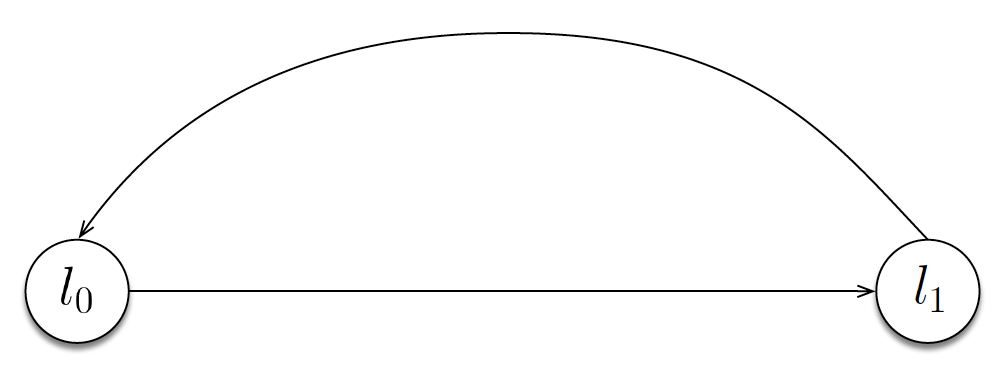
\includegraphics[width=1.0\textwidth]{notation/diagram1.png}
\caption{}
\label{Algo2Result2}
\end{figure}

The initial location $l_0$ has a bold border; the initial condition $x_0$ will not be given in the diagram as multiple parameterizations of $x_0$ may be of interest. Hence, the diagram is representing a unique \textit{system} but not necessarily one specific instantiation of the system.

\begin{figure}[H]
\centering
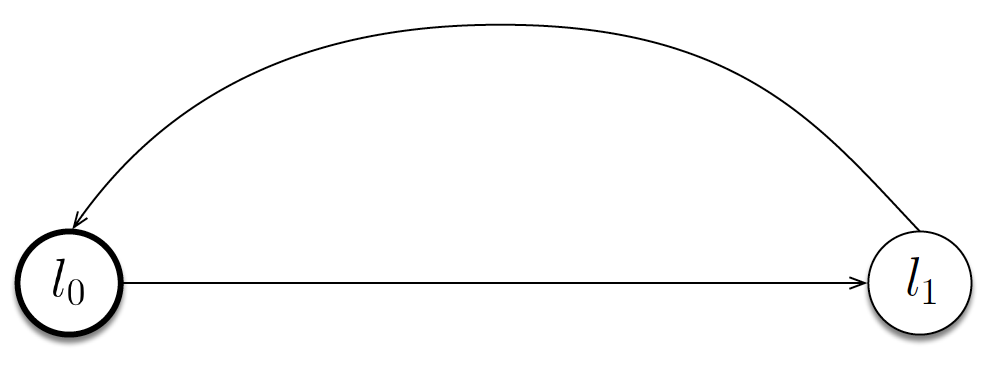
\includegraphics[width=1.0\textwidth]{notation/diagram2.png}
\caption{}
\label{diagram2}
\end{figure}


Forced transitions are represented with solid lines while dotted lines indicate unforced transitions as shown in Figure \ref{fig:forcedUnforced}.

\begin{figure}[H]
\centering
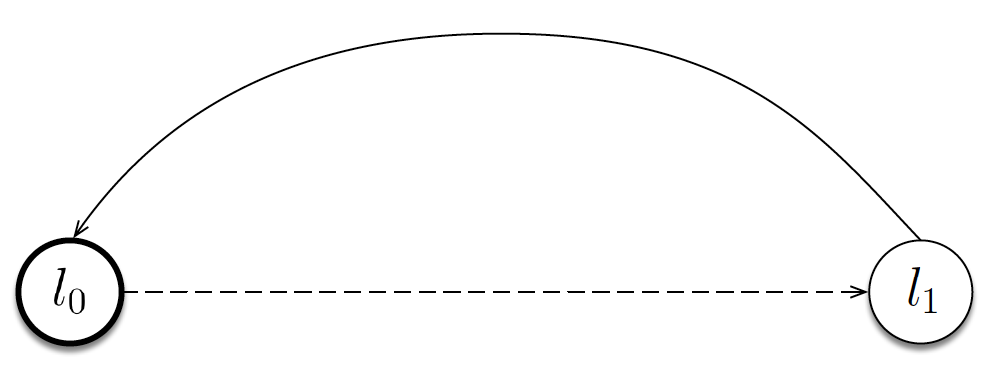
\includegraphics[width=1.0\textwidth]{notation/diagram3.png}
\caption{}
\label{fig:forcedUnforced}
\end{figure}

The vector field associated with a location is given within a box adjacent to the location itself. It can be given in vectorized or component-wise form:

\begin{figure}[H]
\centering
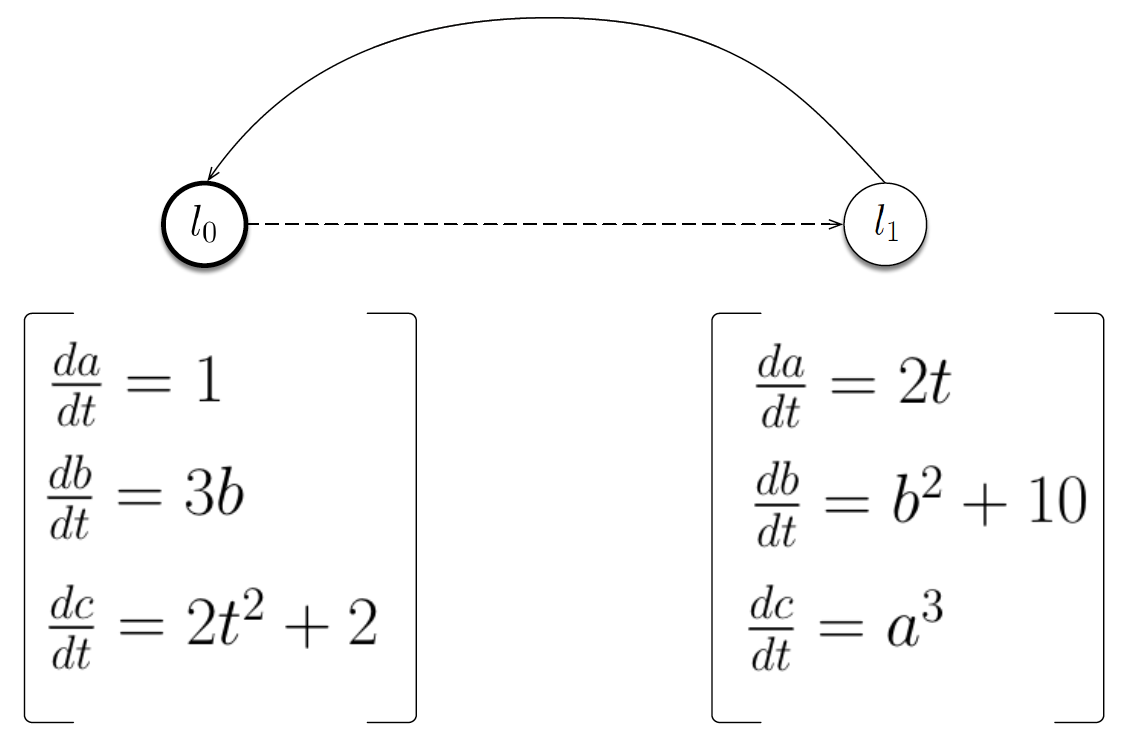
\includegraphics[width=1.0\textwidth]{notation/diagram4.png}
\caption{}
\label{Algo2Result2}
\end{figure}

\begin{figure}[H]
\centering
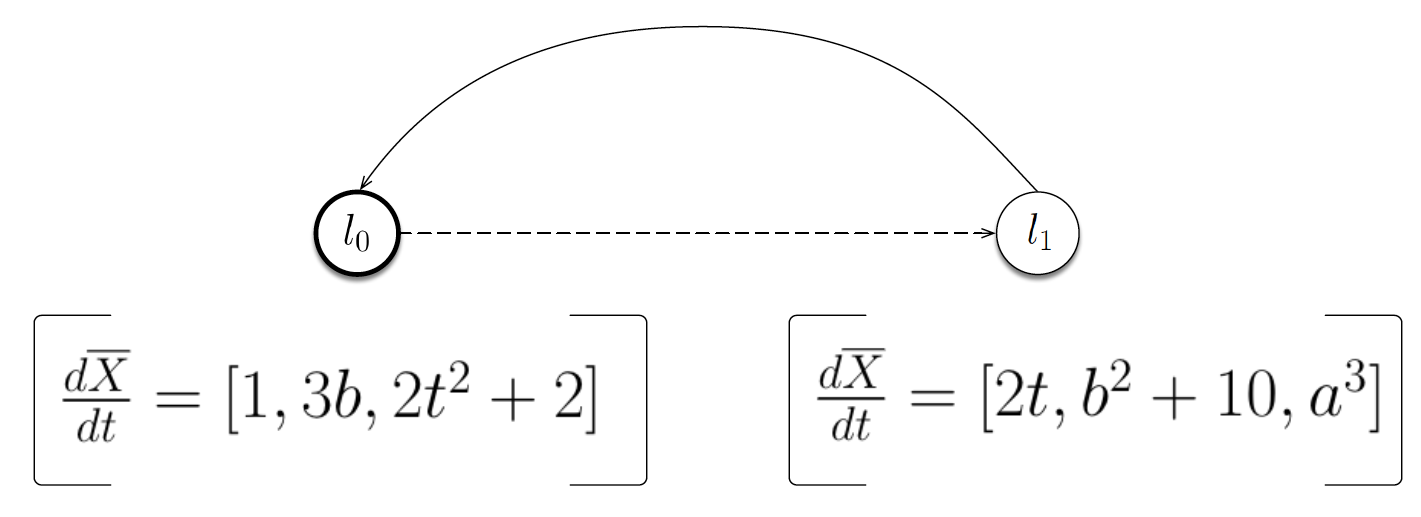
\includegraphics[width=1.0\textwidth]{notation/diagram5.png}
\caption{}
\label{Algo2Result2}
\end{figure}


Vectorized notation may also be used in conjunction with component-wise notation:

\begin{figure}[H]
\centering
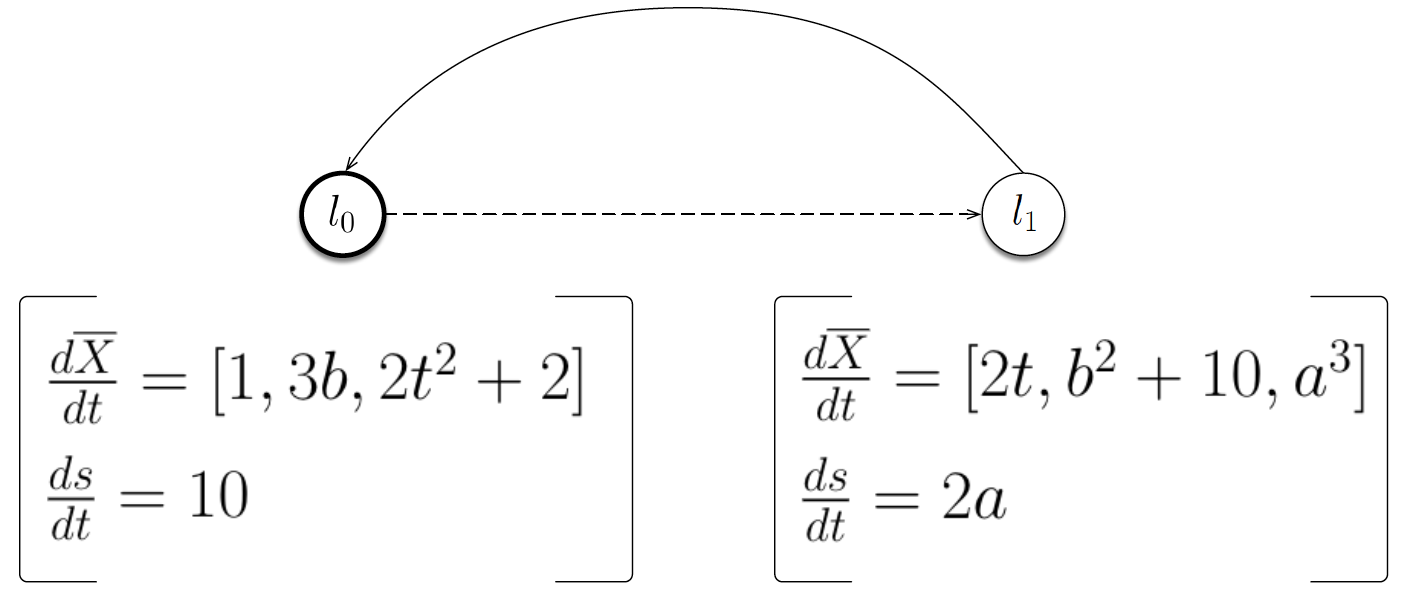
\includegraphics[width=1.0\textwidth]{notation/diagram6.png}
\caption{}
\label{Algo2Result2}
\end{figure}

It is not necessary to explicitly list the continuous variables in $X$; the variables for which no dynamics are given are redundant when seeking a unique representation for the state-space of the system; omitting them does not reduce the expressibility of the language accepted by the automaton.

The guards on a transition are given as bracketed systems of inequalities, adjacent to the edge representing the transition. The bracketed system also contains the resets and the event label associated with the transition:

\begin{figure}[H]
\centering
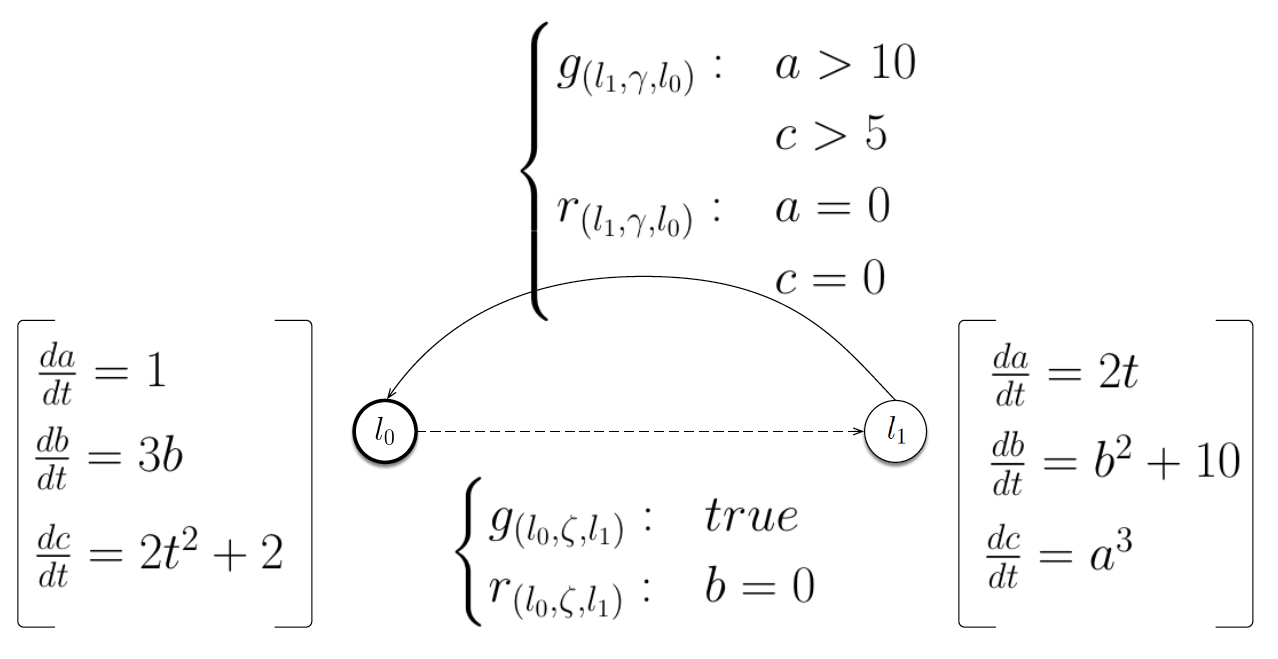
\includegraphics[width=1.0\textwidth]{notation/diagram7.png}
\caption{}
\label{Algo2Result2}
\end{figure}

Many of the automata presented in this work have a finite, but indeterminate, number of locations. It is important, then, to be able to compactly express automata that would otherwise be very large in expanded graphical notation upon enumerating all locations $l_0, l_1, ..., l_n$.

The notation for doing so is as follows:

\begin{figure}[H]
\centering
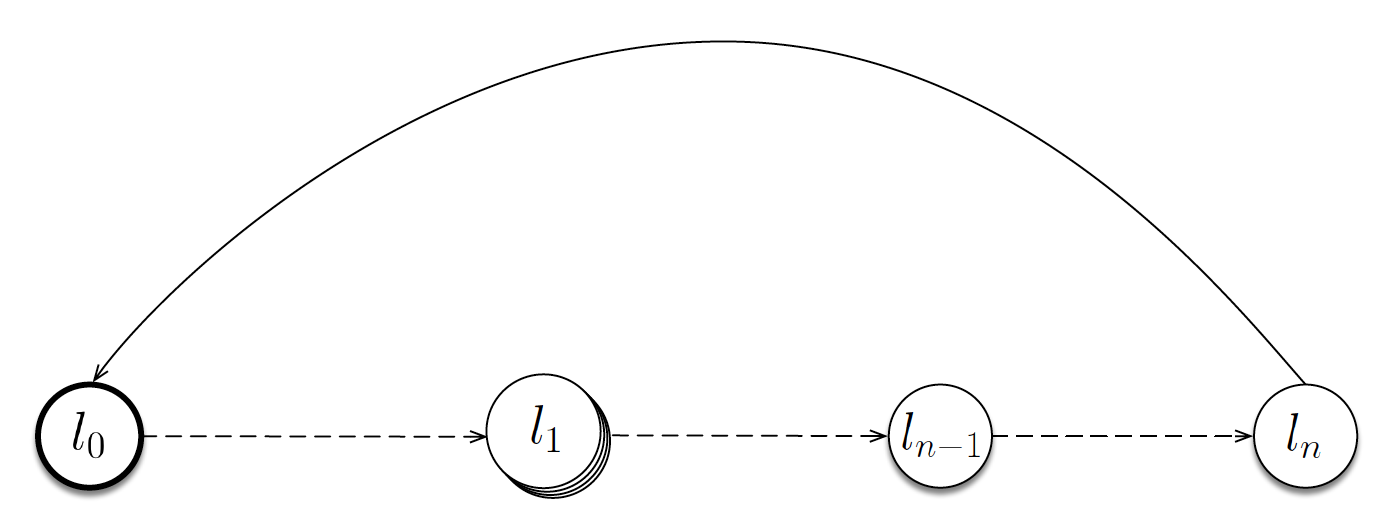
\includegraphics[width=1.0\textwidth]{notation/diagram8.png}
\caption{}
\label{Algo2Result2}
\end{figure}

The locations $l_3$ up to $l_{n-2}$ are ``hidden" under location $l_2$. While concise, it is impossible to explicitly define transitions, guards, and resets between such locations. Hence, this representation should only be used when the properties of the transitions can be inferred from the transition immediately preceding ($l_0$ to $l_1$) and succeeding ($l_{n-2}$ to $l_{n-1}$).

In the two automata that follow, the transitions, guards, resets, and dynamics on the obscured locations should be able to be reasonably inferred from the transitions and dynamics that are explicitly given:

\begin{figure}[H]
\centering
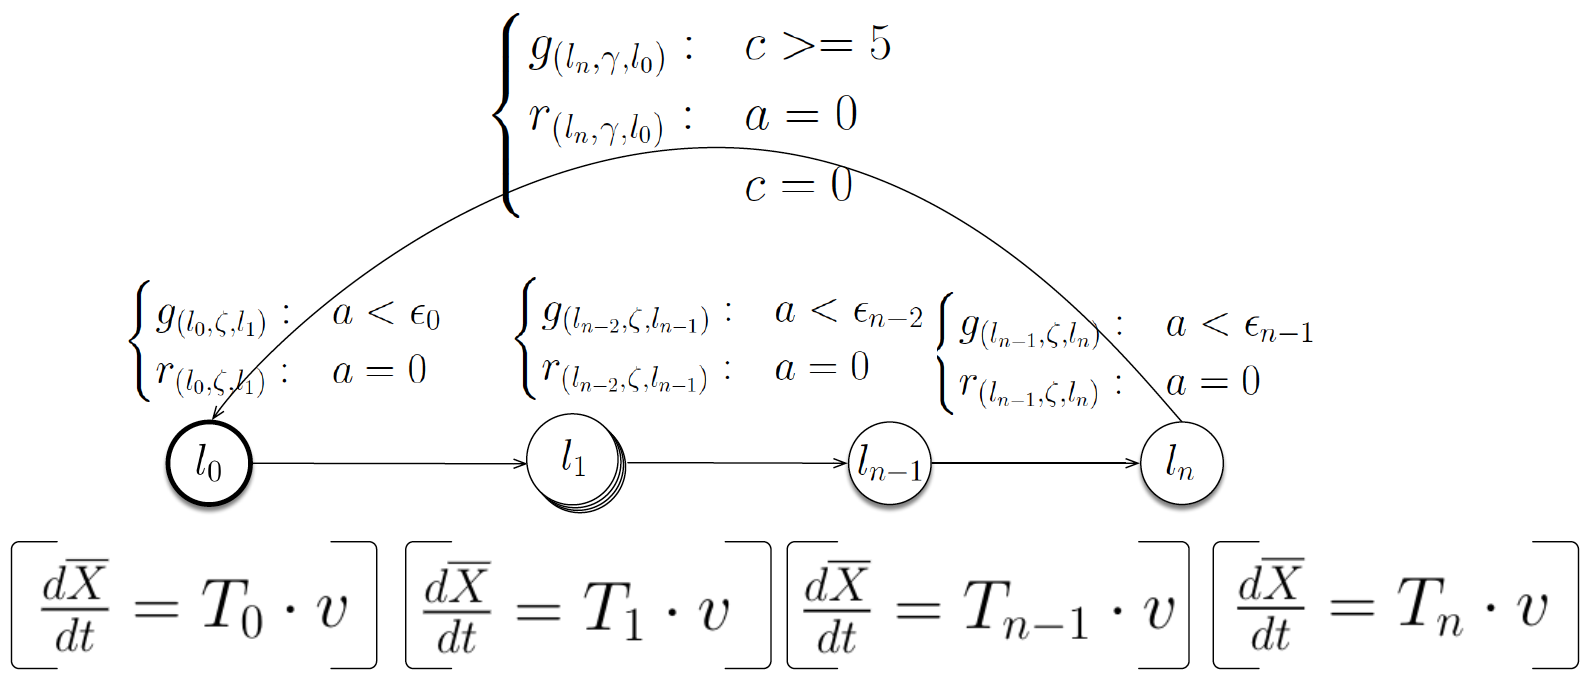
\includegraphics[width=1.0\textwidth]{notation/diagram9.png}
\caption{}
\label{Algo2Result2}
\end{figure}

\begin{figure}[H]
\centering
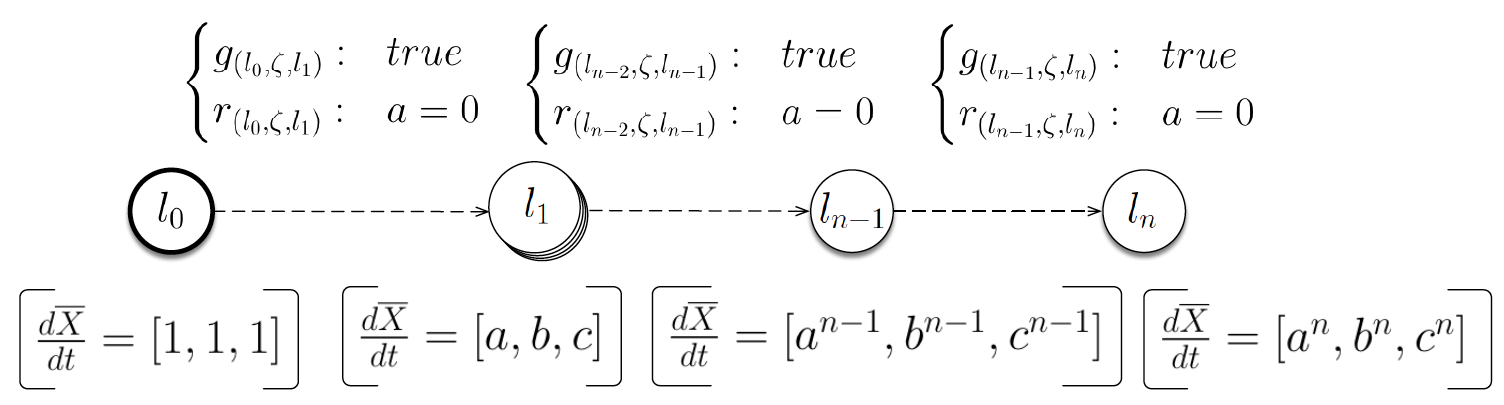
\includegraphics[width=1.0\textwidth]{notation/diagram10.png}
\caption{}
\label{Algo2Result2}
\end{figure}

For visual clarity, some transitions from multiple locations to a singular location may be merged, in the event that they have the same guards and resets:

% automata with merged transition